\documentclass[a4paper, 12pt]{article}
% packages
\usepackage{amssymb}
\usepackage[fleqn]{mathtools}
\usepackage{tikz}
\usepackage{enumerate}
\usepackage{bussproofs}
\usepackage{xcolor}
\usepackage[margin=1.3cm]{geometry}
\usepackage{logicproof}
\usepackage{diagbox}
\usepackage{listings}
\usepackage{graphicx}
\usepackage{lstautogobble}
\usepackage{hyperref}
\usepackage{multirow}
\usetikzlibrary{arrows, shapes.gates.logic.US, circuits.logic.US, calc, automata, positioning}

% shorthand for verbatim
\catcode`~=\active
\def~#1~{\texttt{#1}}

% code listing
\lstdefinestyle{main}{
    numberstyle=\tiny,
    breaklines=true,
    showspaces=false,
    showstringspaces=false,
    tabsize=2,
    numbers=left,
    basicstyle=\ttfamily,
    columns=fixed,
    fontadjust=true,
    basewidth=0.5em,
    autogobble,
    xleftmargin=3.0ex,
    mathescape=true
}
\newcommand{\dollar}{\mbox{\textdollar}} %
\lstset{style=main}

% augmented matrix
\makeatletter
\renewcommand*\env@matrix[1][*\c@MaxMatrixCols c]{%
\hskip -\arraycolsep
\let\@ifnextchar\new@ifnextchar
\array{#1}}
\makeatother

% ceiling / floor
\DeclarePairedDelimiter{\ceil}{\lceil}{\rceil}
\DeclarePairedDelimiter{\floor}{\lfloor}{\rfloor}

% custom commands
\newcommand{\indefint}[2]{\int #1 \, \mathrm{d}#2}
\newcommand{\defint}[4]{\int_{#1}^{#2} #3 \, \mathrm{d}#4}
\newcommand{\dif}[2]{\frac{\mathrm{d}#1}{\mathrm{d}#2}}
\newcommand{\limit}[2]{\displaystyle{\lim_{#1 \to #2}}}
\newcommand{\summation}[3]{\sum\limits_{#1}^{#2} #3}
\newcommand{\intbracket}[3]{\left[#3\right]_{#1}^{#2}}
\newcommand{\ulsmash}[1]{\underline{\smash{#1}}}

\newcommand{\powerset}[0]{\wp}
\renewcommand{\emptyset}[0]{\varnothing}

\newcommand{\unaryproof}[2]{\AxiomC{#1} \UnaryInfC{#2} \DisplayProof}
\newcommand{\binaryproof}[3]{\AxiomC{#1} \AxiomC{#2} \BinaryInfC{#3} \DisplayProof}
\newcommand{\trinaryproof}[4]{\AxiomC{#1} \AxiomC{#2} \AxiomC{#3} \TrinaryInfC{#4} \DisplayProof}

% no indent
\setlength\parindent{0pt}

% reasoning proofs
\usepackage{ltablex}
\usepackage{environ}
\keepXColumns
\NewEnviron{reasoning}{
    \begin{tabularx}{\textwidth}{rlX}
        \BODY
    \end{tabularx}
}
\newcommand{\proofline}[3]{$(#1)$ & $#2$ & \hfill #3 \smallskip \\}
\newcommand{\proofarbitrary}[1]{& take arbitrary $#1$ \smallskip \\}
\newcommand{\prooftext}[1]{\multicolumn{3}{l}{#1} \smallskip \\}
\newcommand{\proofmath}[3]{$#1$ & = $#2$ & \hfill #3 \smallskip \\}
\newcommand{\prooftherefore}[1]{& $\therefore #1$ \smallskip \\}
\newcommand{\proofbc}[0]{\prooftext{\textbf{Base Case}}}
\newcommand{\proofis}[0]{\prooftext{\textbf{Inductive Step}}}

% reasoning er diagrams
\newcommand{\nattribute}[4]{
    \node[draw, state, inner sep=0cm, minimum size=0.2cm, label=#3:{#4}] (#1) at (#2) {};
}
\newcommand{\mattribute}[4]{
    \node[draw, state, accepting, inner sep=0cm, minimum size=0.2cm, label=#3:{#4}] (#1) at (#2) {};
}
\newcommand{\dattribute}[4]{
    \node[draw, state, dashed, inner sep=0cm, minimum size=0.2cm, label=#3:{#4}] (#1) at (#2) {};
}
\newcommand{\entity}[3]{
    \node[] (#1-c) at (#2) {#3};
    \node[inner sep=0cm] (#1-l) at ($(#1-c) + (-1, 0)$) {};
    \node[inner sep=0cm] (#1-r) at ($(#1-c) + (1, 0)$) {};
    \node[inner sep=0cm] (#1-u) at ($(#1-c) + (0, 0.5)$) {};
    \node[inner sep=0cm] (#1-d) at ($(#1-c) + (0, -0.5)$) {};
    \draw
    ($(#1-c) + (-1, 0.5)$) -- ($(#1-c) + (1, 0.5)$) -- ($(#1-c) + (1, -0.5)$) -- ($(#1-c) + (-1, -0.5)$) -- cycle;
}
\newcommand{\relationship}[3]{
    \node[] (#1-c) at (#2) {#3};
    \node[inner sep=0cm] (#1-l) at ($(#1-c) + (-1, 0)$) {};
    \node[inner sep=0cm] (#1-r) at ($(#1-c) + (1, 0)$) {};
    \node[inner sep=0cm] (#1-u) at ($(#1-c) + (0, 1)$) {};
    \node[inner sep=0cm] (#1-d) at ($(#1-c) + (0, -1)$) {};
    \draw
    ($(#1-c) + (-1, 0)$) -- ($(#1-c) + (0, 1)$) -- ($(#1-c) + (1, 0)$) -- ($(#1-c) + (0, -1)$) -- cycle;
}

% actual document
\begin{document}
    \section*{CO150 - Graphs and Algorithms}
        \subsection*{Prelude}
            The content discussed here is part of CO150 - Graphs and Algorithms (Computing MEng); taught by Iain Phillips, in Imperial College London during the academic year 2018/19. The notes are written for my personal use, and have no guarantee of being correct (although I hope it is, for my own sake). This should be used in conjunction with the notes.
        \subsection*{14th January 2019}
            Introduction to the structure of the course;
            \begin{enumerate}[{Part} I:]
                \itemsep0em
                \item Graphs
                \item Graph Algorithms
                \item Algorithm Analysis
                \item Introduction to Complexity
            \end{enumerate}
            An example graph with a real life application;
            \begin{center}
                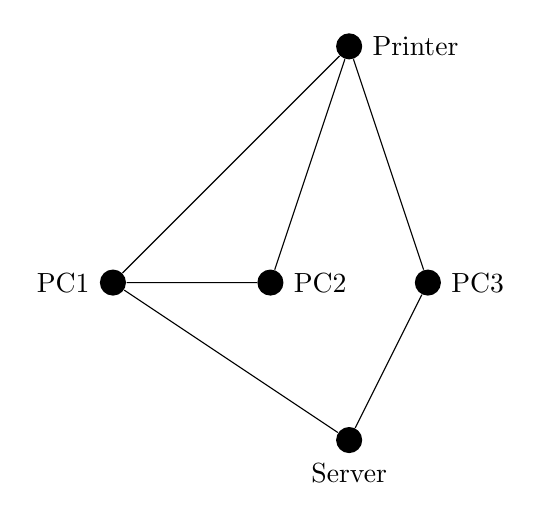
\begin{tikzpicture}
                    \node[circle, fill=black, label=right:PC2] (pc2) at (0, 0) {};
                    \node[circle, fill=black, label=left:PC1] (pc1) at (-2, 0) {};
                    \node[circle, fill=black, label=below:Server] (server) at (1, -2) {};
                    \node[circle, fill=black, label=right:PC3] (pc3) at (2, 0) {};
                    \node[circle, fill=black, label=right:Printer] (print) at (1, 3) {};

                    \draw
                    (print) -- (pc1)
                    (print) -- (pc2)
                    (print) -- (pc3)
                    (server) -- (pc1)
                    (server) -- (pc3)
                    (pc1) -- (pc2);
                \end{tikzpicture}
            \end{center}
            Note how all the PCs are directly connected to the printer, but PC2 can only reach the server through PC1. On the other hand, we can create a more general graph to display some features that may be less common;
            \begin{center}
                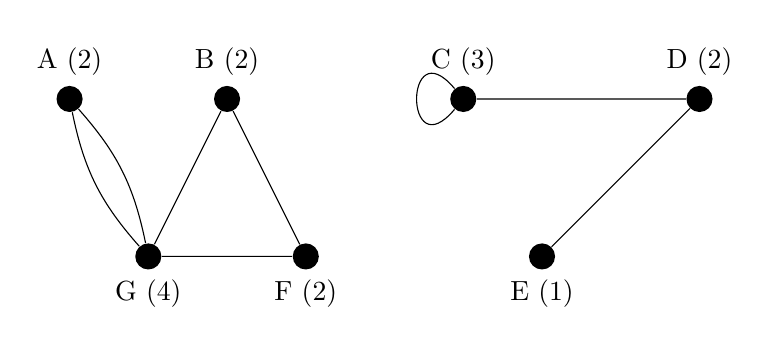
\begin{tikzpicture}
                    \node[circle, fill=black, label=above:A (2)] (a) at (0, 0) {};
                    \node[circle, fill=black, label=above:B (2)] (b) at (2, 0) {};
                    \node[circle, fill=black, label=above:C (3)] (c) at (5, 0) {};
                    \node[circle, fill=black, label=above:D (2)] (d) at (8, 0) {};
                    \node[circle, fill=black, label=below:E (1)] (e) at (6, -2) {};
                    \node[circle, fill=black, label=below:F (2)] (f) at (3, -2) {};
                    \node[circle, fill=black, label=below:G (4)] (g) at (1, -2) {};

                    \draw
                    (b) -- (g)
                    (g) -- (f)
                    (f) -- (b)
                    (c) -- (d)
                    (d) -- (e)
                    (a) edge[bend left=15] node{} (g)
                    (a) edge[bend right=15] node{} (g)
                    (c) edge[loop, out=230, in=130, distance=1cm] (c);
                \end{tikzpicture}
            \end{center}
            Note that this isn't actually two graphs; it's \textbf{disconnected components}. Between A, and G, there are two \textbf{parallel arcs / edges}, and C has \textbf{loop} with itself. I will continue to refer to this graph as the "example", for the remainder of this section, since it displays properties which we may want to analyse later.
            \medskip

            We can say that the left subgraph is robust, as it will remain connected against a single failure. However, the right subgraph isn't robust, as a failure between C, and D, or between E, and D would cause one of the nodes to become disconnected. We can then remedy this by adding a connection between C, and E.
            \medskip

            In the graph drawn above, the degrees are also specified - which is the number of arcs connected to it. Note that the degree of C is 3, as we count loops twice for consistency reasons. The sum of the degrees is 16, which is double the number of arcs (8). This is because each arc is counted twice (where it starts, and where it ends), therefore the sum of the degrees is always even. From that, we can then infer that the number of odd nodes (C, and E in our case) must be even. This is trivial to prove with arithmetic.
            \subsubsection*{Subgraphs}
                We can say that $G_1$ is a subgraph of $G_2$ if both of the following criteria apply;
                \begin{itemize}
                    \itemsep0em
                    \item $\text{nodes}(G_1) \subseteq \text{nodes}(G_2)$
                    \item $\text{arcs}(G_1) \subseteq \text{arcs}(G_2)$
                \end{itemize}
                A full (induced) subgraph occurs when we have a set of nodes, $X$, such that $X \subseteq \text{nodes}(G)$. Every connection between the nodes in $X$, that was present in $G$, exists in $G[X]$. Then $G^\prime$ is a full subgraph of $G$, if $G^\prime = G[X]$ for some $X$. For example, let $X = \{A, B, G\}$, from the example graph, then we have the following induced subgraph;
                \begin{center}
                    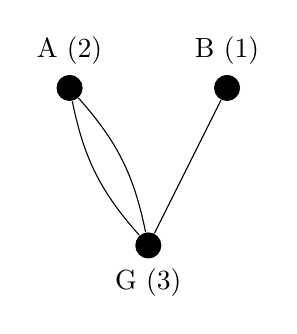
\begin{tikzpicture}
                        \node[circle, fill=black, label=above:A (2)] (a) at (0, 0) {};
                        \node[circle, fill=black, label=above:B (1)] (b) at (2, 0) {};
                        \node[circle, fill=black, label=below:G (3)] (g) at (1, -2) {};

                        \draw
                        (b) -- (g)
                        (a) edge[bend left=15] node{} (g)
                        (a) edge[bend right=15] node{} (g);
                    \end{tikzpicture}
                \end{center}
                If we have some subgraph $G^\prime$, and $\text{nodes}(G^\prime) = \text{nodes}(G)$, then it $G^\prime$ spans $G$.
            \subsubsection*{Adjacency Matrix}
                For the entry in the matrix $a_{i,j}$, it represents the number of arcs thast connect $i$ to $j$. In an undirected graph, this matrix is symmetric (such that $a^\top = a$). In our example, we're doing the rows, and columns, alphabetically. It's also important to note that we count each loop twice in a diagonal entry. We can determine the degree of a node by taking the sum of its respective row (or column), and find the number of arcs by taking the sum of all the values in the matrix, and then halving it.
                \begin{center}
                    $\begin{matrix}
                        \text{A} \\
                        \text{B} \\
                        \text{C} \\
                        \text{D} \\
                        \text{E} \\
                        \text{F} \\
                        \text{G}
                    \end{matrix}$$\begin{bmatrix}
                        0 & 0 & 0 & 0 & 0 & 0 & 2 \\
                        0 & 0 & 0 & 0 & 0 & 1 & 1 \\
                        0 & 0 & 2 & 1 & 0 & 0 & 0 \\
                        0 & 0 & 1 & 0 & 1 & 0 & 0 \\
                        0 & 0 & 0 & 1 & 0 & 0 & 0 \\
                        0 & 1 & 0 & 0 & 0 & 0 & 1 \\
                        2 & 1 & 0 & 0 & 0 & 1 & 0
                    \end{bmatrix}$
                \end{center}
            \subsubsection*{Adjacency Lists}
                You'll notice that in our graph, we have a lot of 0s, which makes it less efficient to store as an adjacency matrix; especially if we don't require random access to the degrees. We tend to use $n$ to represent the number of nodes (vertices), and $m$ to represent the number of arcs (edges). You'll note that the size of this is $\leq n + 2m$ (as we have $n$ nodes on the left, and each arc is counted twice, except for loops). Therefore, we can say a graph is sparse if $2m \ll n^2$. Since certain algorithms we work with only look at the arcs incident to a given node, a linked list will be better for sparse graphs.
                \begin{center}
                    \begin{tabular}{|c|@{ $\rightarrow$ }l|}
                        \hline
                        A & G, G \\
                        \hline
                        B & F, G \\
                        \hline
                        C & C, D \\
                        \hline
                        D & C, E \\
                        \hline
                        E & D \\
                        \hline
                        F & B, G \\
                        \hline
                        G & A, A, B, F \\
                        \hline
                    \end{tabular}
                \end{center}
            \subsubsection*{Big-Oh Notation}
                I'm too lazy to write out the example, but the idea is that we ignore constant factors, and only consider the most significant term; for example, we could summarise some algorithm that takes $3n^4 + 2n - 4631$ to run as $O(n^4)$. This has significant advantages, since it allows us to abstract away from the implementation / hardware specifics, and instead focus on the factors which determine growth.
            \subsubsection*{Isomorphism}
                In general, an isomorphism is a bijection that preserves connections. While the two graphs drawn below appear fairly different, they are isomorphic. Mapping from the left, to the right, we know that $3 \mapsto D$, simply because they are the only nodes with degree 2. It's also evident that $1 \mapsto B$, as it's the only node which has two sets of parallel arcs coming out of it. However, it doesn't matter which of 4, or 2, maps to $A$, or $C$. Therefore, we can say $4 \mapsto A, 2 \mapsto C$, or $4 \mapsto C, 2 \mapsto A$.
                \begin{center}
                    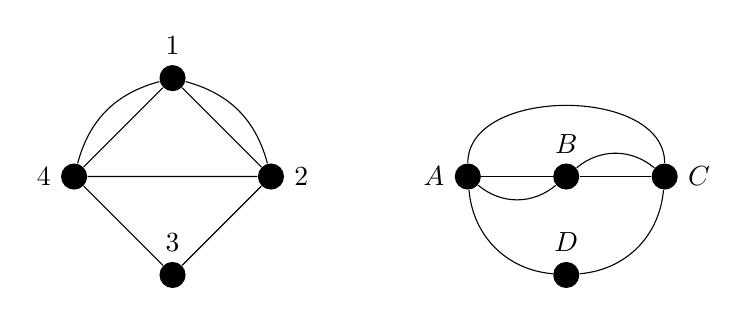
\begin{tikzpicture}[x=1.25cm, y=1.25cm]
                        \node[circle, fill=black, label=above:1] (1) at (0, 1) {};
                        \node[circle, fill=black, label=right:2] (2) at (1, 0) {};
                        \node[circle, fill=black, label=above:3] (3) at (0, -1) {};
                        \node[circle, fill=black, label=left:4] (4) at (-1, 0) {};
                        \draw
                        (4) -- (2)
                        (4) -- (1)
                        (4) -- (3)
                        (1) -- (2)
                        (2) -- (3)
                        (4) edge[bend left=30] (1)
                        (1) edge[bend left=30] (2);

                        \node[circle, fill=black, label=left:$A$] (A) at (3, 0) {};
                        \node[circle, fill=black, label=above:$B$] (B) at (4, 0) {};
                        \node[circle, fill=black, label=right:$C$] (C) at (5, 0) {};
                        \node[circle, fill=black, label=above:$D$] (D) at (4, -1) {};

                        \draw
                        (A) -- (B)
                        (B) -- (C)
                        (A) edge[bend left=90] (C)
                        (A) edge[bend right=40] (D)
                        (D) edge[bend right=40] (C)
                        (A) edge[bend right=40] (B)
                        (C) edge[bend right=40] (B);
                    \end{tikzpicture}
                \end{center}
                While we're able to check this fairly easily by simply looking at the graph, a computer would have to rearrange the LHS' adjacency matrix to the RHS' (or vice versa).
                \medskip

                Given two graphs, $G, G^\prime$, an isomorphism from $G$ to $G^\prime$ consists of two bijections (one-to-one mapping), as well as an additional restriction;
                \begin{itemize}
                    \itemsep0em
                    \item $f : \text{nodes}(G) \mapsto \text{nodes}(G^\prime)$
                    \item $g : \text{arcs}(G) \mapsto \text{arcs}(G^\prime)$
                    \item if $a \in \text{arcs}(G)$, with endpoints $n_1, n_2$, then the endpoints of $g(a)$ are $f(n_1), f(n_2)$ (see the diagram below for a visual example).
                \end{itemize}
                \begin{center}
                    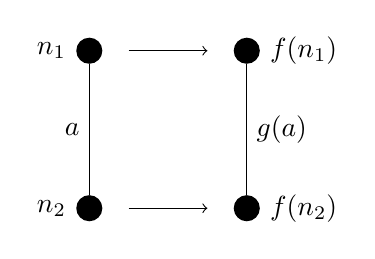
\begin{tikzpicture}
                        \node[circle, fill=black, label=left:$n_1$] (n1) at (0, 0) {};
                        \node[circle, fill=black, label=left:$n_2$] (n2) at (0, -2) {};
                        \node[circle, fill=black, label=right:$f(n_1)$] (fn1) at (2, 0) {};
                        \node[circle, fill=black, label=right:$f(n_2)$] (fn2) at (2, -2) {};
                        \draw
                        (n1) edge[left] node{$a$} (n2)
                        (fn1) edge[right] node{$g(a)$} (fn2)
                        ($(n1) + (0.5, 0)$) edge[->] ($(fn1) + (-0.5, 0)$)
                        ($(n2) + (0.5, 0)$) edge[->] ($(fn2) + (-0.5, 0)$);
                    \end{tikzpicture}
                \end{center}
                In order to confirm whether two graphs are isomorphic, the easiest approach is to first check the obvious; whether the number of arcs, nodes, and loops are the same, as well as the degrees of the nodes. If any of these are different, then the graphs cannot be isomorphic. However if they pass all the tests, then we can attempt to find a bijection on the nodes.
        \subsection*{17th January 2019}
            \subsubsection*{Complexity}
                Generally, the process of determining whether two graphs are isomorphic is computationally expensive, hence it has a high complexity. A naive approach would be to check all the permutations, which would then lead to a time complexity of $O(n!)$, which is worse than even exponential ($O(2^n)$).
            \subsubsection*{Automorphisms}
                An automorphism on $G$ is an isomorphism from $G$ to itself. Every graph has at least one automorphism (the identity). Consider the following graph;
                \begin{center}
                    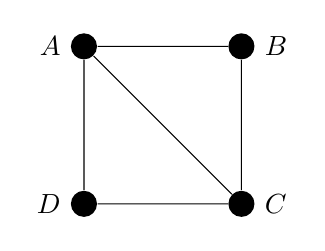
\begin{tikzpicture}
                        \node[circle, fill=black, label=left:$A$] (a) at (0, 0) {};
                        \node[circle, fill=black, label=right:$B$] (b) at (2, 0) {};
                        \node[circle, fill=black, label=right:$C$] (c) at (2, -2) {};
                        \node[circle, fill=black, label=left:$D$] (d) at (0, -2) {};
                        \draw
                        (a) -- (b) -- (c) -- (d) -- (a) -- (c);
                    \end{tikzpicture}
                \end{center}
                We can do the following method to find the number of automorphisms;
                \begin{itemize}
                    \itemsep0em
                    \item fix a node, $B$, it can go to where $D$ is, or stay (2 possibilities)
                    \item take the next node $A$, it can either stay where it is, or go to where $C$ is (2 possibilities), now fix it
                    \item take the next node $C$, it can only stay where it is, as it can't go to $D$ since $D$ isn't connected to $B$, nor does it have a degree of 3 (1 possibility), now fix it
                    \item finally $D$ can only stay where it is (1 possibility)
                    \item multiply all the possibilities, and we have 4 automorphisms
                \end{itemize}
            \subsubsection*{Planar Graphs}
                We can say a graph is planar if it can be drawn such that no arcs cross. Any non-planar graph contains $K_5$, or $K_{3,3}$ as a subgraph homeomorphic. We can say that two graphs are \textbf{homeomorphic} if they can be obtained by a series of operations such that an arc $x - y$, is replaced by two arcs $x - z$, and $z - y$. For example, the two graphs below are homeomorphic.
                \begin{center}
                    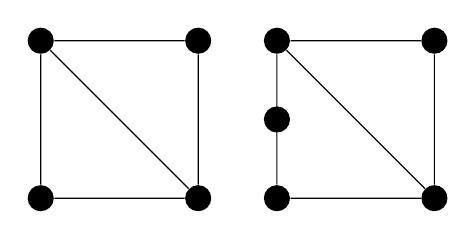
\begin{tikzpicture}
                        \node[circle, fill=black] (a) at (0, 0) {};
                        \node[circle, fill=black] (b) at (2, 0) {};
                        \node[circle, fill=black] (c) at (2, -2) {};
                        \node[circle, fill=black] (d) at (0, -2) {};
                        \draw
                        (a) -- (b) -- (c) -- (d) -- (a) -- (c);

                        \node[circle, fill=black] (a) at (3, 0) {};
                        \node[circle, fill=black] (b) at (5, 0) {};
                        \node[circle, fill=black] (c) at (5, -2) {};
                        \node[circle, fill=black] (d) at (3, -2) {};
                        \node[circle, fill=black] (e) at (3, -1) {};
                        \draw
                        (a) -- (b) -- (c) -- (d) -- (a) -- (c);
                    \end{tikzpicture}
                \end{center}
                There is a linear time algorithm to check whether a graph is planar; however in this case linear time means $O(n + m)$, with the previous definitions.
                \medskip

                Any planar graph splits the plane into regions, which are referred to as faces; the graph below splits it into 6 faces (including the outside region). With a graph $G$ that has $N$ nodes, $A$ arcs, and $F$ faces, Euler's formula states $F = A - N + 2$ for any connected planar graph.
                \begin{center}
                    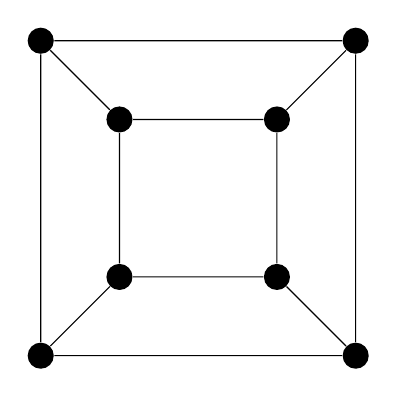
\begin{tikzpicture}
                        \node[circle, fill=black] (a) at (0, 0) {};
                        \node[circle, fill=black] (b) at (2, 0) {};
                        \node[circle, fill=black] (c) at (2, -2) {};
                        \node[circle, fill=black] (d) at (0, -2) {};
                        \node[circle, fill=black] (e) at (-1, 1) {};
                        \node[circle, fill=black] (f) at (3, 1) {};
                        \node[circle, fill=black] (g) at (3, -3) {};
                        \node[circle, fill=black] (h) at (-1, -3) {};
                        \draw
                        (a) -- (b) -- (c) -- (d) -- (a) -- (e) -- (f) -- (g) -- (h) -- (e)
                        (b) -- (f)
                        (c) -- (g)
                        (d) -- (h);
                    \end{tikzpicture}
                \end{center}
            \subsubsection*{Graph Colouring}
                Any (literal, real-life) map can be convereted into a simple planar graph by letting the countries represent nodes, and joining them if they are neighbours. This newly generated graph is known as the dual graph. We can say some graph $G$ is $k$-colourable, if the nodes of $G$ can be coloured with no more than $k$ colours, therefore every simple planar graph is 4-colourable.
            \subsubsection*{Bipartite Graphs}
                We can say a graph is bipartite if we can partition nodes($G$), into two sets $X$, and $Y$, such that no two nodes of $X$ are joined, and likewise for $Y$. A graph is biparite $\Leftrightarrow$ it is 2-colourable.
            \subsubsection*{Paths, and Connectedness}
                A path in a graph is a sequence of adjacent arcs, although normally described by the nodes that we pass through. A path is called \textbf{simple} if it doesn't repeat nodes, and a graph is \textbf{connected} if there is a path joining any two nodes.
                \medskip

                We can define a relation on nodes($G$) by $x \sim y \Leftrightarrow$ there is a path from $x$ to $y$. This is an equivalence relation, as we can prove it's reflexive, symmetric, and transitive.
                \begin{itemize}
                    \itemsep0em
                    \item $\forall x \in \text{nodes}(G) [x \sim x]$, $x$ is trivially connected to itself, hence it is reflexive
                    \item $\forall x,y \in \text{nodes}(G) [x \sim y \Rightarrow y \sim x]$, as we are working on an undirected graph, this follows trivially
                    \item $\forall x,y,z \in \text{nodes}(G) [x \sim y \land y \sim z \rightarrow x \sim z]$, follows trivially by definition of paths
                \end{itemize}
                A cycle (circuit) is a special type of path that finishes where it starts, has at least one arc, and doesn't reuse an arc. A graph which doesn't have cycles is \textbf{acyclic}.
        \subsection*{21st January 2019}
            \subsubsection*{Euler Paths / Circuits}
                An Euler path is a special type of path where each arc is used exactly once, and an Euler circuit is a cycle which uses each arc exactly once (therefore an EC is an EP which finishes at the start node). A connected graph has an EP $\Leftrightarrow$ there are 0, or 2 odd nodes, and there is an EC $\Leftrightarrow$ there are no odd nodes.
                \medskip

                We can justify it by saying that any intermediate node (ones which aren't the start node) have to be entered, and exited the same number of times (otherwise it wouldn't be an intermediate) node. Therefore, if 2 nodes of odd degree, then it follows that we start from one, and end on the other.
                \medskip

                Consider the following nodes; $n$, $n^\prime$ being the start, and end (the odd nodes of the path), and arbitrary intermediate nodes $i$. Start at $n$, and keep going until we can go no further ($n^\prime$). If we've stopped at $n$, then there must be a spare arc, as we've started, and 'ended' at an odd node. If we stop at some arbitrary $i \neq n^\prime$, then we've still got more arcs, since $i$ is even.
            \subsubsection*{Hamiltonian Path / Circuits}
                A Hamiltonian path is one that visits each node exactly once, and similarly a Hamiltonian circuit returns to the start node. For this, we will only consider simple graphs, since we won't ever follow a loop, or a parallel arc. In order for there to be a HP, we need a connected graph, and for a HC to exist, each node must have a degree $\geq 2$. To determine whether a circuit exists, we can take a brute force approach, since a circuit is really just a permutation on the set of nodes; such that for $n$ nodes, we have $\pi : \{1, ..., n\} \mapsto \{1, ..., n\}$. However, for this to be a circuit, we need $\pi(i)$ to be adjacent to $\pi(i + 1)$, and so on. As we have $n!$ possible circuits, this is far too slow. There exists a dynamic programming approach that reduces this to $O(n^22^n)$, but that is still exponential. Compared to EPP, which has $O(n^2)$ time. HCP has been shown to be NP-complete, and are therefore not solvable in polynomial time.
            \subsubsection*{Trees}
                A tree is an acyclic connected graph (whether we specify it's rooted, or nonrooted, depends on the author). The root of $G$ is a distinguished node. Assuming a rooted graph, the depth of a node $x$ is the distance along the unique path from the root to $x$. If $x$ isn't the root node, the parent of $x$ is the node directly before it in the path from the root to $x$. The depth of tree is the maximum of the depths of all its nodes.
                \medskip

                A spanning tree of a graph $G$, is a tree, $T$, such that $\text{nodes}(T) = \text{nodes}(G)$, and $\text{arcs}(T) \subseteq \text{arcs}(G)$. The spanning trees are not necessarily unique.
            \subsubsection*{Directed Graphs}
                While we generally cover undirected graphs in this course, it makes sense in some applications for the arcs to be directed. For each $a \in \text{arcs}(G)$, it is associated with an \textbf{ordered} pair of nodes. In diagrams, these are shown with arrows. In a path for $a_1, ..., a_n$, the source of $a_{i + 1}$, must match the target of $a_i$. We define the indegree as the number of arcs entering, and likewise the outdegree is the number of args leaving. For any directed graph, the sum of the indegree of all nodes, and the outdegree of all nodes is equal to the number of arcs. We say a directed graph is strongly connected if there exists a path between any two nodes in $G$.
        \subsection*{24th January 2019}
            \subsubsection*{Tree Traversal Algorithms}
                The two types of traversal covered in this course are depth-first search (DFS), and breadth-first search (BFS). While they are similar in many ways, they also have quite a few differences.
                \medskip

                In depth first search, we choose one of the adjacent nodes to the start; from there, we then spawn another depth first search. This is done recursively until there aren't any more (unvisited) adjacent nodes. At this point, the spawned DFS returns back to the parent node, where it checks the next adjacent node (normally ordered by how the adjaceny list / matrix is stored). It does this until we have visited all of the nodes, and then returns back all the way to the start.
                \medskip

                In contrast to DFS, breadth-first search goes through all the adjacent nodes, and then goes deeper. This means that we only check the nodes adjacent to the ones adjacent to the start node, after all of the nodes directly adjacent to the start node have been visited.
                \medskip

                You'll note that the distance between 1, and 8, is 5 in DFS, but only 1 in BFS. In BFS, the depth of any node is its distance from the start. However, both generate spanning trees on $G$.
                \begin{center}
                    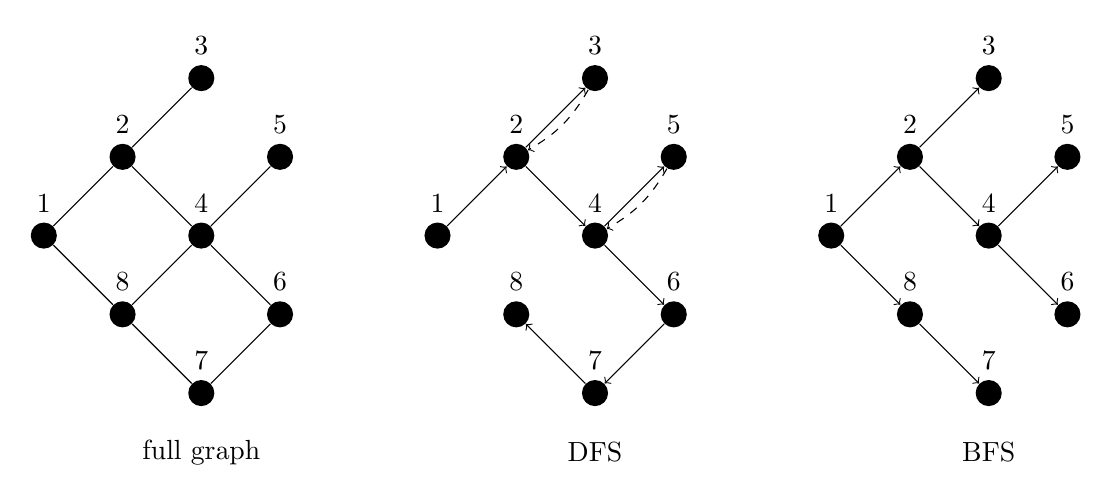
\begin{tikzpicture}
                        \node[] () at (2, -2.75) {full graph};
                        \node[] () at (7, -2.75) {DFS};
                        \node[] () at (12, -2.75) {BFS};
                        \foreach \x in {0, 1, 2} {
                            \node[circle, fill=black, label=above:1] (1-\x) at (5*\x, 0) {};
                            \node[circle, fill=black, label=above:2] (2-\x) at (1 + 5*\x, 1) {};
                            \node[circle, fill=black, label=above:3] (3-\x) at (2 + 5*\x, 2) {};
                            \node[circle, fill=black, label=above:4] (4-\x) at (2 + 5*\x, 0) {};
                            \node[circle, fill=black, label=above:5] (5-\x) at (3 + 5*\x, 1) {};
                            \node[circle, fill=black, label=above:6] (6-\x) at (3 + 5*\x, -1) {};
                            \node[circle, fill=black, label=above:7] (7-\x) at (2 + 5*\x, -2) {};
                            \node[circle, fill=black, label=above:8] (8-\x) at (1 + 5*\x, -1) {};
                        }
                        \draw
                        (1-0) -- (2-0) -- (3-0)
                        (1-0) -- (8-0) -- (7-0) -- (6-0) -- (4-0) -- (5-0)
                        (8-0) -- (4-0) -- (2-0);

                        \draw
                        (1-1) edge[->] (2-1)
                        (2-1) edge[->] (3-1)
                        (3-1) edge[bend left=15, ->, dashed] (2-1)
                        (2-1) edge[->] (4-1)
                        (4-1) edge[->] (5-1)
                        (5-1) edge[bend left=15, ->, dashed] (4-1)
                        (4-1) edge[->] (6-1)
                        (6-1) edge[->] (7-1)
                        (7-1) edge[->] (8-1);

                        \draw
                        (1-2) edge[->] (2-2)
                        (1-2) edge[->] (8-2)
                        (2-2) edge[->] (3-2)
                        (2-2) edge[->] (4-2)
                        (8-2) edge[->] (7-2)
                        (4-2) edge[->] (5-2)
                        (4-2) edge[->] (6-2);
                    \end{tikzpicture}
                \end{center}
                In order to formalise this, let us consider the graph to be traversed as an adjaceny list, a boolean array of nodes (which are visited), and the parent is the parent node in the search tree. The output will be the nodes visited in order.
                \begin{lstlisting}
                    procedure dfs(x):
                      visited[x] = true
                      print x
                      for y in adj[x]:
                        if not visited[y]:
                          parent[y] = x;
                          dfs(y)
                          # at this point, control is returned to x
                          # we don't need the parent in this case, but other applications may use it
                \end{lstlisting}
                The running time of DFS is $O(n + m)$, therefore it's linear. However, this implementation may have some overhead due to recursion.
                \begin{lstlisting}
                    procedure bfs(x):
                      visited[x] = true
                      print[x]
                      enqueue(x, Q)
                      while not isEmpty(Q):
                        y = front(Q)
                        for z in adj[y]:
                          if not visited[z]:
                            visited[z] = true
                            print z
                            parent[z] = y
                            enqueue(z, Q)
                        dequeue(Q)
                \end{lstlisting}
                The size of the queue represents the breadth of the front. Once again, the time complexity is $O(n + m)$.
            \subsubsection*{Applications of Traversal}
                The algorithms used above also work on non-connected graphs. If we analyse the set of visited nodes, and see that it isn't the same as the set of all nodes, then it is clear that the graph is not connected. As such, we have an $O(n + m)$ algorithm for detecting non-connected graphs.
                \medskip

                We can trivially say that a graph has a cycle if it has $\geq n$ arcs. Alternatively, we can use DFS; if we encounter a node that has already been visited (other than by backtracking), then it has a cycle.
                \medskip

                It's also trivial to modify BFS to find the distance of each node, by having a running counter. Due to how BFS is implemented, we can also extract the shortest path from ~y~; as ~y, parent[y], parent[parent[y]], ..., start~.
            \subsubsection*{Weihted Graphs}
                We can associate a cost with each arc on a network. We can define a weighted graph as a graph, $G$, with a weight function $W : \text{arcs}(G) \mapsto \mathbb{R}^+$. With weights, we're able to consider the following problems; finding an MST (minimum spanning tree), finding shortest paths, and finding a shortest circuit.
                \medskip

                We're only going to consider simple graphs, as there is no point in taking a loop if we're trying to minimise cost, nor is there any point in taking the more expensive arc in a parallel arc.
            \subsubsection*{Prim's Algorithm}
                We can say that $T$ is a minimum spanning tree for $G$m if $T$ is a spanning tree for $G$, and no other spanning tree for $G$ has a smaller weight. Once again, MSTs do not have to be unique.
                \medskip

                The main idea in Prim's algorithm is to add the shortest arc that will extend the tree. This is an example of a greedy algorithm, which gives a short-term advantage byt may not be the best overall (it is in this case). At any stage in Prim's algorithm, we have three types of nodes; tree nodes (which are already part of the MST), candidate nodes - which are fringe nodes adjacent to a tree node, and the rest are unseen nodes. At the start, all nodes are unseen.
                \begin{center}
                    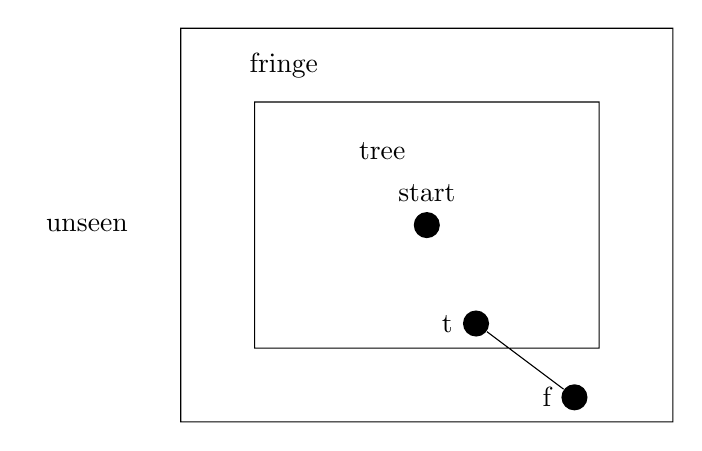
\begin{tikzpicture}[x=1.25cm, y=1.25cm]
                        \node[circle, fill=black, label=above:start] () at (2.5, -2) {};
                        \node[circle, fill=black, label=left:t] (t) at (3, -3) {};
                        \node[circle, fill=black, label=left:f] (f) at (4, -3.75) {};
                        \node[] () at (1, -0.375) {~fringe~};
                        \node[] () at (2, -1.25) {~tree~};
                        \node[] () at (-1, -2) {~unseen~};
                        \draw
                        (0, 0) -- (5, 0) -- (5, -4) -- (0, -4) -- cycle
                        (0.75, -0.75) -- (4.25, -0.75) -- (4.25, -3.25) -- (0.75, -3.25) -- cycle
                        (t) -- (f);
                    \end{tikzpicture}
                \end{center}
                The general idea is to pick a random node (doesn't matter which, as all nodes will be in the MST by definition). This is now the start node, and therefore part of the MST (hence classified as ~tree~). Now classify all the nodes adjacent to this node as ~fringe~. While the fringe isn't empty, select the arc with minimum length between a tree node $t$, and a fringe node $f$. Classify $f$ as ~tree~, and add the arc $(t, f)$ to the tree. Reclassify all the unseen nodes adjacent to $f$ as ~fringe~.
                \medskip

                The while loop is executed roughly $n$ times, as it will be executed for each node. However, in the worst case, when we're selecting a minimum arc, that takes $n + m$. Therefore, we can calculate this to be an $O(n(n + m))$ algorithm. This is a more naive approach, we can improve this by choosing candidate arcs; as we're avoiding redoing work. If we consider a parent function, such that the parent of $f$ (~fringe~) is $t$ (~tree~), such that the arc $(t, f)$ has the least weight. This can be summarised in two parts; first the initialsation, and then the execution of the algorithm;
                \begin{lstlisting}
                    tree[start] = true
                    for x in adj[start]:
                      fringe[x] = true
                      parent[x] = start
                      weight[x] = $W$(start, x)
                    while not isEmpty(fringe):
                      select f such that weight[f] is minimum
                      fringe[f] = false
                      tree[f] = true
                      for y in adj[f]:
                        if not tree[y]:
                          if fringe[y]:
                            # updating arcs if we can get a lower weight
                            if $W$(f, y) < weight[y]:
                              weight[y] = $W$(f, y)
                              parent[y] = f
                          else:
                            # we haven't seen y yet
                            # this can probably be shortend with the above
                            fringe[y] = true
                            weight[y] = $W$(f, y)
                            parent[y] = f
                \end{lstlisting}
                We're still iterating through the loop $n$ times. During the while loop, we're checking whether the fringe is empty (an $O(n)$ operation), finding the minimum fringe (also an $O(n)$ operation), and updating the candidate arc (if needed), which is constant time. Therefore the inner loop has a time complexity of $O(n)$, hence the overall algoithm has a complexity of $O(n^2)$. In the worst case, $m$ can be as large as $n^2$, which would be problematic in the first implementation.
                \medskip

                However, we have a greedy algorithm, and therefore need to prove its correctness. Let us represent the trees constructed at each iteration as $T_0, T_1, ..., T_k, T_{k + 1}...$; where $T_0$ is juts the initial start node, and you get $T_{k + 1}$ from $T_k$, by adding some arc $a_{k + 1}$. Hence it follows that $T_k$ has $k + 1$ nodes (by induction, probably). With this algorithm, we will end up with $n$ nodes, by definition of a spanning tree, therefore we end up returning $T_{n - 1}$.
                \medskip

                The goal here is to now show each $T_k$ is a subgraph of an MST $T^\prime$ of $G$. Trivially, in the base case $T_0$, it has one node, and no arcs, therefore $T_0 \subseteq T^\prime$.
                \medskip

                Assume that $T_k \subseteq T^\prime$, where $T^\prime$ is an MST of $G$. Let there be some node in the tree $x$, a node in the fringe $y$, and an arc joining them $a_{k + 1}$. We can now consider both cases; if $a_{k + 1} \in \text{arcs}(T^\prime)$, then $T_{k + 1} \subseteq T^\prime$, and is trivial. However, suppose that $a_{k + 1} \notin \text{arcs}(T^\prime)$, there still has to be a path in $T^\prime$ from $x$, to $y$ (by properties of a spanning tree). Therefore, we can form a cycle through some other tree node $x^\prime$, to a fringe node $y^\prime$, through some arc $a$ (such that we can connect $y$, and $y^\prime$). As Prim's chose $a_{k + 1}$, instead of $a$, there we can deduce that $W(a_{k + 1}) \leq W(k)$, and therefore $W(T^{\prime\prime}) \leq W(T^\prime))$. However, since all MSTs have the same weight by definition, we can say that $W(T^{\prime\prime}) = W(T^\prime))$. Also, $T_{k + 1} \subseteq T^{\prime\prime}$, therefore the induction step is complete.
                \medskip

                We can also implement Prim's with a priority queue. The PQ requires us to have some key of $x$, for each item $x$. In this case, we will likely use the weight of the candidate arc. We have the following operations on PQ;
                \begin{itemize}
                    \itemsep0em
                    \item ~Q = PQCreate()~
                    \item ~isEmpty(Q)~
                    \item ~insert(Q, x)~
                    \item ~getMin(Q)~
                    \item ~deleteMin(Q)~
                    \item ~decreaseKey(Q, x, newkey)~
                \end{itemize}
                The implemenation is as follows;
                \begin{lstlisting}
                    Q = PQCreate()
                    for x in nodes$(G)$:
                      key[x] = $\infty$ # some arbitrary large number
                      parent[x] = null
                      insert(Q, x)
                    decreaseKey(Q, start, 0)
                    while not isEmpty(Q):
                      f = getMin(Q)
                      deleteMin(Q)
                      tree[f] = true
                      for y in adj[f]:
                        if not tree[y]: # therefore in Q
                          if $W$(f, y) < key[y]:
                            decreaseKey(Q, y, $W$(f, y))
                            parent[y] = f
                \end{lstlisting}
                With a priority queue of length $N$, all operations have time complexity log($N$) (other than ~isEmpty~, and ~getMin~, which are constant time), with a good implementation. Overall, we have a time complexity of $O(m \text{log}(n))$, given that $n < m$. In a dense graph, classic Prim is better.
        \subsection*{28th January 2019}
            \subsubsection*{Kruskal's Algorithm}
                An even greedier approach is to take the shortest arc that hasn't been included in the tree, except for ones that would cause a cycle. In intermediate stages, we have a forest (which is an acyclic graph), and not a tree (a connected acyclic graph).
                \medskip

                In our implementation, we need to do two things; look at each arc in ascending order (we can either sort the arcs right at the start, or use a priority queue). We will also need to use \textbf{dynamic equivalence classes}, which prevents adding arcs that would cause cycles. We can generate equivalence classes if they belong to the same connected tree, and an arc $(x, y)$ can only be added if $x$, and $y$ are in different equivalence classes. If the arc is added, the classes are merged.
                \medskip

                We can use the \textbf{Union-Find} data type to implement these DECs. Let each set have a leader element, which represents the set. We can \textbf{find} the leader of the equivalence class, and union (merge) two classes (discussion of the implemention is in the next section);
                \begin{itemize}
                    \itemsep0em
                    \item ~sets = UFCreate(n)~ \hfill creates a family of singleton sets, with ~find(sets, x) = x~
                    \item ~x' = find(sets, x)~ \hfill finds the leader ~x'~ of ~x~ within ~sets~
                    \item ~union(sets, x, y)~ \hfill merges the sets led by ~x~, and ~y~, and choose one to be the leader
                \end{itemize}
                Consider $G$ with $n$ nodes numbered $[1, n]$;
                \begin{lstlisting}
                    Q = PQCreate() # arcs of $G$ with the weights as keys
                    sets = UFCreate(n)
                    F = $\emptyset$
                    while not isEmpty(Q):
                      (x, y) = getMin(Q)
                      deleteMin(Q)
                      x' = find(sets, x)
                      y' = find(sets, y)
                      if x' != y':
                        add (x, y) to F
                        union(sets, x', y')
                \end{lstlisting}
                With a weighted union (non-binary tree) implemenation of Union-Find, we have a time complexity of find being $O(\text{log}(n))$, and a union of $O(1)$;
                \begin{itemize}
                    \itemsep0em
                    \item $O(m)$ inserts for the PQ, which takes $O(m\text{log}(m))$
                    \item $O(m)$ ~getMins~, ~deleteMins~, which both take $O(m\text{log}(m))$
                    \item $O(m)$ ~finds~, which takes $O(m\text{log}(n)$
                    \item $O(n)$ ~unions~, which takes $O(n)$
                \end{itemize}
                Assuming $m \geq n$, as it's normally the case, the overal time is $O(m\text{log}(m))$. However, we know that the number of arcs in a simple graph is bounded by $n^2$, hence the complexity is $O(m\text{log}(n))$ which is the same as a PQ implementation of Prim's.
        \subsection*{31st January 2019}
            \subsubsection*{Union-Find Implementations}
                A naive implemention for the union-find is to store an array of leader nodes, where it initially stores itself as its leader. Finding is $O(1)$, but union will be $O(n)$, which means our implementation of Kruskal's will be $O(n^2)$.
                \medskip

                Instead of taking the naive approach, we can consider it as a non-binary tree, with the root node being the leader for the equivalence class. When two trees are merged, with leaders ~x~, and ~y~, we either set ~parent[x] = y~, or vice versa. This now makes a merging operation $O(1)$, which is much better. However, finding the parent will now involve traversing up the ~parent~ chain, which would be $O(n)$ in the worst case (on a tree where it's basically a linked list). This still keeps Kruskal's at $O(n^2)$, which isn't an improvement.
                \medskip

                The goal for us now is to minimise the depth of the tree, by taking a weighted union instead of some arbitrary choice. The rule for a weighted union is to append the tree of lower size (number of nodes, not depth), to the one of greater size. Storing, and updating, size is a very simple operation. By the weighted union, the depth of a tree of size $k$ is $\leq \floor{\text{log}(k)}$.
            \subsubsection*{Path Compression}
                We can reduce the union-find complexity for Kruskal's to $O((n + m)\text{log}^*(n))$, where $\text{log}^*(n)$ is an extremely slow-growing function, such that it's $\leq 5$ for any $n$ we might use. The idea is to set the parent of some node we're finding by the root node as follows;
                \begin{lstlisting}
                    procedure cfind(x):
                      y = parent[x]
                      if y == x:
                        root = x
                      else:
                        root = cfind(y)
                        if root != y: # path compression
                          parent[x] = root # path compression
                      return root
                \end{lstlisting}
            \subsubsection*{Comparison}
                We can refer to the table below to summarise the time complexities of each of the algorithms we're referring to. On dense graphs, where $m$ has order $n^2$ (is large), then Kruskal's gives a complexity of $O(n^2\text{log}(n))$, therefore classic Prim's is better. ON the other hand, where $m$ is small, around the order of $n\text{log}(n)$, then Kruskal's or PQ Prim's is better, as we have $O(n\text{log}^2(n))$.
                \begin{center}
                    \begin{tabular}{l|r}
                        algorithm & time complexity \\
                        \hline
                        Kruskal & $O(m\text{log}(n))$ \\
                        Prim with binary heap PQ & $O(m\text{log}(n))$ \\
                        Classic Prim & $O(n^2)$
                    \end{tabular}
                \end{center}
            \subsubsection*{Fibonacci Heaps}
                If we implemented a PQ with a Fibonacci heap instead of a binary heap, we have all constant time operations (other than ~deleteMin~, which would have a complexity of $O(\text{log}(n))$. The complexity of Prim's with a Fibonacci heap PQ is $O(m + n\text{log}(n))$, however the memory usage, as well as constant factors, can be higher, therefore a binary heap might still be preferred.
            \subsubsection*{Shortest Path Problem}
                Given we have a weighted graph $G$, and nodes $S$, and $F$, representing start, and finish respectively, we have an $O(n^2)$ algorithm to find the shortest path of a single pair developed by Dijkstra. There is also an algorithm by Floyd, which finds all the shortest paths between any pairs, in $O(n^3)$ time.
                \medskip

                As Dijkstra's is closely related to Prim's, we can use the same diagram from before, with some modifications (not just because I'm too lazy to draw another one with TikZ). Once again, the nodes are classified into ~tree~, ~fringe~, and ~unseen~. However, we modify it by saying that we've already computed the shortest path from the start node, to all the ~tree~ nodes - the path given by the tree. For the ~fringe~ nodes, we know the shortest path using the tree, although this path can be improved as the tree grows (similar to the inductive step in the proof for Prim's). However, instead of choosing the shortest candidate arc, we choose the shortest distance from the staff.
                \begin{center}
                    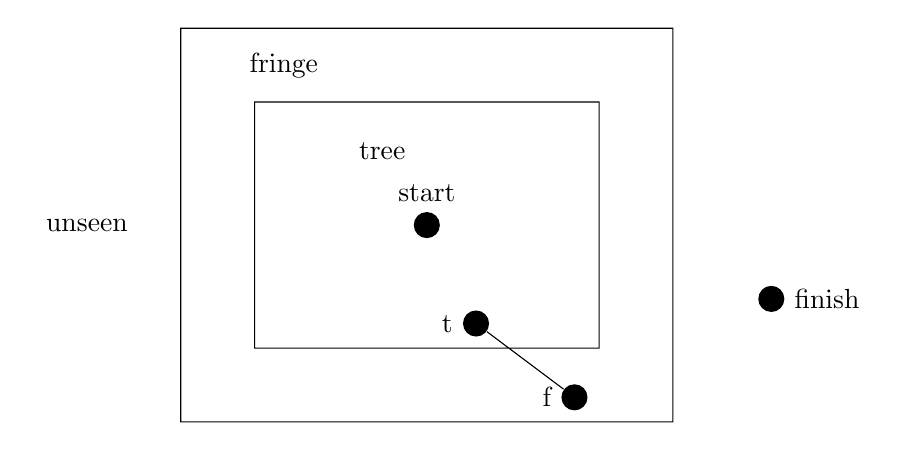
\begin{tikzpicture}[x=1.25cm, y=1.25cm]
                        \node[circle, fill=black, label=above:start] () at (2.5, -2) {};
                        \node[circle, fill=black, label=left:t] (t) at (3, -3) {};
                        \node[circle, fill=black, label=left:f] (f) at (4, -3.75) {};
                        \node[circle, fill=black, label=right:finish] (fin) at (6, -2.75) {};
                        \node[] () at (1, -0.375) {~fringe~};
                        \node[] () at (2, -1.25) {~tree~};
                        \node[] () at (-1, -2) {~unseen~};
                        \draw
                        (0, 0) -- (5, 0) -- (5, -4) -- (0, -4) -- cycle
                        (0.75, -0.75) -- (4.25, -0.75) -- (4.25, -3.25) -- (0.75, -3.25) -- cycle
                        (t) -- (f);
                    \end{tikzpicture}
                \end{center}
                The implementation fro this is similar to Prim's algorithm, but we also need to store its parent node, and the distance of the shortest path known. At any stage, the next node to be added is the fringe nede with the smallest distance from the start. The fringe is then updated, possibly improving the shortest path. Once again, we can keep checking parents to obtain the path we'e taken.
                \begin{lstlisting}
                    tree[start] = true
                    for x in adj[start]:
                      fringe[x] = true
                      parent[x] = start
                      distance[x] = $W$(start, x)
                    while not tree[finish] and not isEmpty(fringe):
                        select f where distance[f] is minimum
                        fringe[f] = false
                        tree[f] = true
                        for y in adj[f]:
                          if not tree[y]:
                            if fringe[y]:
                              if distance[f] + $W$(f, y) < distance[y]:
                                # updating distance if we have a better option
                                distance[y] = distance[f] + $W$(f, y)
                                parent[y] = f
                            else:
                              fringe[y] = true
                              distance[y] = distance[f] + $W$(f, y)
                              parent[y] = f
                    return distance[finish]
                \end{lstlisting}
                As it's merely a light modification on Prim's, we can easily justify that the running time is $O(n^2)$. We can prove termination, as we're increasing the tree each iteration. Once again, we can implement this with a PQ as such;
                \begin{lstlisting}
                    Q = PQCreate()
                    for x in nodes($G$):
                      key[x] = $\infty$
                      parent[x] = null
                      insert(Q, x)
                    decreaseKey(Q, start, 0)
                    while not tree[finish] and not isEmpty(Q):
                      f = getMin(Q)
                      deleteMin(Q)
                      tree[f] = true
                      for y in adj[f]:
                        if not tree[y]:
                          if key[f] + $W$(f, y) < key[y]:
                            decreaseKey(Q, y, key[f] + $W$(f, y))
                            parent[y] = f
                \end{lstlisting}
                Once again, the complexity is the same, with either the binary heap, or the Fibonacci heap implementation.
        \subsection*{4th Febuary 2019}
            \subsubsection*{A$^*$ Algorithm}
                Djikstra's algorithm omits any sense of direction, and expands outwards until we reach the finish node. A$^*$ modifies this by allowing for some heuristic function $h(x)$ by underestimating the distance from any node to the finish node. On a map, we could say that $h$ represents the Euclidean distance between any two cities.
                \medskip

                We can calculate the cost of going to a node as $F(x) = g(x) + h(x)$, where $g(x)$ is what we defined as the distance between the target node, and the start node. Given a start node, we calculate the 'cost' of the node by taking the $F$ values of them, and then we select the smallest one. We then add that node, $x$, to the tree. At this point, we can then consider the nodes adjacent to $x$, and calculate their costs, by using the same method. This checks the smallest cost nodes, that aren't already checked, but we will end up saving time since the heuristic function adds a bias towards the nodes that are heading in the direction of the finish. In order for a heuristic function to be considered consistent, it needs to fulfill the follwoing criteria;
                \begin{itemize}
                    \itemsep0em
                    \item for any two adjacent nodes, $x, y$, we have $h(x) \leq W(w, y) + h(y)$
                    \item $h(~finish~) = 0$
                \end{itemize}
                Consistency is a stronger property than a function being admissible (if $h(x) \leq $ the weight of the shortest path from $x$ to the finish). We can solve this trivially with the consistency criteria, by setting $y = ~finish~$, as we'd then have $h(x) \leq W(x, ~finish~)$.
                \medskip
                The set of tree nodes is often referred to as the \textbf{closed set}, and the set of fringe is the \textbf{open} set. If we have a heuristic $h(x) = 0$, albeit useless, then we get Dijkstra's algorithm. Thus we can say that the time complexity of A$^*$ is the same as Djikstra, in the worst case. We can justify correctness similar to Dijkstra's. Our 'invariant' is that if the node $x$ is a ~tree~, or ~fringe~ node, and not the ~start~, then ~parent[$x$]~ is a tree node. If $x$ is a tree node, then $g(x)$ is the length of the shortest path (once again, not including ~start~). However, if $x$ is a fringe node, then $g(x)$ is the length of the shortest path, where all nodes except $x$ are tree nodes.
                \medskip

                Let us assume that we have a different, shorter path $P$, which may exist outside the tree nodes. Then it follows that $\text{len}(P) < g(x)$. Let there be some $y$ which is the first node in that isn't part of the tree to be on $P$, and $P_1$ be the path from $~start~$ to $y$, and $P_2$ be the path from $y$ to $x$. We know that $F(y) = g(y) + h(y)$, by definition. Therefore $\leq g(y) + \text{len}(P_2) + h(x)$, by the consistent property of $h$. And also that $\leq \text{len}(P_1) + \text{len}(P_2) + h(x) = \text{len}(P) + h(x)$. As we've assumed that it has a shorter path, it follow that it must be $< g(x) + h(x) = F(x)$. Therefore $F(y) < F(x)$, but that contradicts our choice of $x$, since we chose the lowest $F$.
                \medskip

                For the sake of completeness; this is the algorithm implemented with a PQ;
                \begin{lstlisting}
                    Q = PQCreate()
                    for x in nodes($G$):
                      g[x] = $\infty$
                      key[x] = $\infty$
                      parent[x] = null
                      insert(Q, x)
                    g[start] = 0
                    decreaseKey(Q, start, g[start] + h[start])
                    while not tree[finish] and not isEmpty(Q):
                      x = getMin(Q)
                      deleteMin(Q)
                      tree[x] = true
                      for y in adj[x]:
                        if not tree[y]:
                          if g[x] + $W$(x, y) < g[y]:
                            g[y] = g[x] + $W$(x, y)
                            decreaseKey(Q, y, g[y] + h[y])
                            parent[y] = x
                \end{lstlisting}
        \subsection*{7th February 2019}
            \subsubsection*{Transitive Closure}
                Let there be some binary relation $R \subseteq X^2$. We can use the definition of transitive closure from \textbf{CO142} (whoops, probably should've done Discrete Structures before trying to learn this module), as $R^+ = \bigcup\limits_{\infty}^{k=1} R^k$.
                \smallskip

                However, instead of using $\infty$, we can use $|X|$ instead, given that $X$ is a finite set. We can interpret $R$ as a directed graph on $G$, where the ordered pairs of $R$ are arcs in $G$, and elements in $X$ are nodes in $G$. Therefore, we can deduce that $R^k(x, y) \Leftrightarrow$ there is a path of length $k$, from $x$ to $y$. Therefore $R^+(x, y) \Leftrightarrow$ there is a path of length $\geq 1$ from $x$ to $y$.
                \medskip

                Assuming we have the set $X = \{1, ..., n\}$, and $A[i, j] = 1$ if $R(i, j)$, otherwise 0, then we have the adjacency matrix $A$ of $G$. Computing $R^k$ is then trivial with matrix multiplication, such that $R^k(i, j) \Leftrightarrow A^k[i, j] > 0$.
                \smallskip

                Then we can simply calculate $B = \summation{k = 1}{n}{A^k}$, which means that $R^+(i, j) \Leftrightarrow B[i, j] > 0$
            \subsubsection*{Warshall's Algorithm}
                Suppose we have nodes $\{1, ..., n\}$. Considering a path $p = x_1, x_2, ..., x_k$ from $x_1$ to $x_k$, we can say that $x_m$ is an intermediate nodes, $\forall m \in [2,k-1]$. We want to look for paths that use nodes $\leq i$ as intermediate nodes. Defining a matrix $B_k[i, j] = 1 \Leftrightarrow$ if there exists a path from $i$ to $j$ that uses only intermediate nodes $\leq k$ (otherwise the value in the matrix is 0).
                \medskip

                Therefore, $B_0[i, j] = A[i, j]$ as we only consider paths of length one, since tehre are no intermediate nodes $\leq 0$. Since $B_n$ allows all possible intermediate nodes, we have all possible paths, therefore $R^+(i, j) \Leftrightarrow B_n[i, j]$.
                \medskip

                Consider how to compute $B_k$ from $B_{k - 1}$. Suppose we have some path $P$ from $i$ to $j$, using intermediate nodes $\leq k$. The path either contains $k$ as an intermediate node, or it doesn't. In the former, $k$ is not an intermediate node, therefore $B_{k - 1}[i, j]$. However, if it is, we only consider when $k$ occurs once (if it repeats, then it's not helpful - we just remove the path between the two $k$s). Then we have some path $i$ to $k$, and another path $k$ to $j$, therefore it follows that $B_{k - 1}[i,  k]$, and also $B_{k - 1}[k, j]$. This has a trivial time complexity of $O(n^3)$, which is much more efficient than the matrix method for closure.
                \begin{lstlisting}
                    input A
                    copy A into B # B = B$_\text{0}$
                    for k = 1 to n:
                      # B = B$_\text{k - 1}$
                      for i = 1 to n:
                        for j = 1 to n:
                            B[i, j] = B[i, j] or (B[i, k] and B[k, j])
                      # B = B$_\text{k}$
                    #B = B$_\text{n}$
                    return B
                \end{lstlisting}
            \subsubsection*{Floyd's Algorithm}
                Returning to the all pairs shortest path problem on some weighted directed graph $G$. This can be solved with a modification of Warshall's. Once again, $G$ has nodes $\{1, ..., n\}$, and an adjacency matrix $A$. We now consider $B_k[i, j]$ to be the length of the shortest path between $i$, and $j$ which has intermediate nodes $\leq k$. If there isn't a path, then let the value be $\infty$. Once again, like with Warshall's, we let $B_n[i, j]$ represent the length of the shortest path between $i$, and $j$. Assume that we know $B_{k - 1}$, and we want to get $B_k$. Suppose there eixsts some shortest path $P$ from $i$ to $j$, using intermediate nodes $\leq k$, with $\text{len}(P) = d$. Once again, if we consider the two cases, the case where $k$ is not in $P$, is trivial, and the second where $k$ is in the path, only occuring once. We can then calculate the length between the two as the minimum of $B_{k-1}[i, j]$, and $B_{k-1}[i, k] + B_{k-1}[k, j]$. If there aren't any shortest paths, then we still get $\infty$. Once again, it has the same time complexity of $O(n^3)$.
                \begin{lstlisting}
                    input A
                    (for all i, j <= n) B[i, j] = 0       if i = j
                                                  A[i, j] if i $\neq$ j and there is an arc (i, j)
                                                  $\infty$        otherwise
                    for k = 1 to n:
                      for i = 1 to n:
                        for j = 1 to n:
                            B[i, j] = min(B[i, j], B[i, k] + B[k, j])
                    return B
                \end{lstlisting}
            \subsubsection*{Dynamic Programming}
                The previous two algorithms are examples of dynamic programming. In dynamic programming, we break down the problem into sub-problems, and the smaller sub-problems are ordered to culminate in the main problem. We move through the smaller sub-problems in order, and solve each sub-problem with the stored results of the previous one (and then storing this result for use by the next one). The main problem is solved as if it were the final sub-problem (deep really).
            \subsubsection*{Travelling Salesman Problem}
                Given some complete weighted graph $(G, W)$, we want to find a way to tour the graph visiting each node exactly once, and travelling the shortest possible distance. We consider complete graphs, as we can construct an 'arc' with an extremely high weight.
                \medskip

                This problem is related to the Hamiltonian Circuit Problem, and the Shortest Path Problem. TSP is NP-complete, and unlikely have a polynomial solution. An improvement on the factorial approach is the Bellman-Held-Karp algorithm (will be written as BHK), which has a running time of $O(n^22^n$).
                \medskip

                Once again, we have $(G, W)$ with nodes $\{1, ..., n\}$. We can fix a start node, say 1 as it doesn't matter where you begin, since the problem would require you to visit all of them anyways. For each $x \neq 1$, and each $S \subseteq \text{nodes}\backslash \{1, x\}$, we can find and store the minimum cost of $C(S, x)$ from node 1 to $x$, using the set of intermediate nodes $S$ (you have to use exactly the set of intermediate nodes).
                \medskip

                We can use this to calculate the solution to TSP as $\text{min}(C(\text{nodes}\backslash \{1, x\}, x)) + W(x, 1)$, by trying each $x \neq 1$. This is done by calculating all $C(S, x)$ in increasing size order, from 0 to $n - 2$ (which is all nodes excluding 1, and $x$). Clearly, with the base case $C(\emptyset, x) = W(1, x)$, as we aren't allowed any intermediate nodes. If we assume that we know $C(S, x)$ for all $S$ of size $k$. Now, consider a set $S^\prime$, with a size of $k + 1$, such that $S^\prime = S \cup \{y\}$, where $y$ is some last node (and $S = S^\prime \backslash \{y\}$), Therefore, it follows that the cost of a path from 1 to $x$ with intermediate nodes $S^\prime$ is $C(S, y) + W(y, x)$, therefore it follows that $C(S^\prime, x) = min(C(S, y)) + W(y, x)$.
                \begin{lstlisting}
                    input ($G$, $W$)
                    choose start $\in$ nodes($G$)
                    for x in nodes \ {start}:
                      c[$\emptyset$, x] = $W$(start, x)
                    # process S in size order
                    for S $\subseteq$ nodes \ {start} with S $\neq \emptyset$
                      for x in nodes \ (S $\cup$ {start}):
                      # find c[S, x]
                      c[S, x] = $\infty$
                      for y in S:
                        c[S, x] = min(c[S \ {y}, y] + $W$(y, x), c[S, x])
                    opt = $\infty$
                    for x in nodes \ {start}:
                      opt = min(c[nodes \ {start, x}, x] + $W$(x, start), opt)
                    return opt
                \end{lstlisting}
                For each subset of ~nodes~, we do $O(n^2)$ the two for loops, with an overall complexity of $O(n^22^n)$.
        \subsection*{11th February 2019}
            \subsubsection*{Approximate Methods for TSP}
                We could easily try a nearest neighbour heuristic for TSP, such that we choose the shortest availabel arc that doesn't violate any rules. This can fail though, since we may fall into a point where we're forced to use an extremely high weight arc.
            \subsubsection*{Toplogical Sorting}
                Suppose there is a list of tasks, with prerequisites (therefore some have to be performed others, and these may allow others to be performed). This is seen as an acyclic, directed graph (if it were cyclic, then there would be a sort of circular dependency). Find a total ordering, such that for nodes $x_1, ..., x_n$, for any $i, j \leq n$, if $j > i$, there is no path from $x_j$ to $x_i$.
                \medskip

                Given a DAG $G$, let $x \leq y \Leftrightarrow$ there is a path from $x$ to $y$, then $\subseteq$ is a (weak) partial ordering, as it's reflexive, transitive, and antisymmetric. If you have a partial ordering $(X, \leq)$, then we can create an acyclic directed graph with nodes $X$, and arcs $\{(x,y) : x \leq y\}$.
                \medskip

                We can perform a toplogical sorting by using DFS, as it inherently finishes with all the nodes reachable from $x$ before we finish with $x$. We can add a node to the end of a sorted list, once we've finished processing it (by exiting the node). In the example below, our visiting order is 1, 2, 5, 6, 3, 4, 6. However, we want to consider the order we exit them, not the order in which we enter. Thus we get the exit order 5, 7, 2, 1, 4, 3, 6. Therefore we end up with the sort 6, 3, 4, 1, 2, 7, 5.
                \begin{center}
                    \begin{minipage}{0.485\textwidth}
                        \begin{lstlisting}
                            procedure dfsts(x):
                              entered[x] = true
                              for y in adj[x]:
                                if entered[y]:
                                  if not exited[y]:
                                    ERROR # cycle
                                else:
                                  parent[y] = x
                                  dfts(y)
                            exited[x] = true
                            ts[index] = x
                            index = index -1
                        \end{lstlisting}
                    \end{minipage} \
                    \begin{minipage}{0.485\textwidth}
                        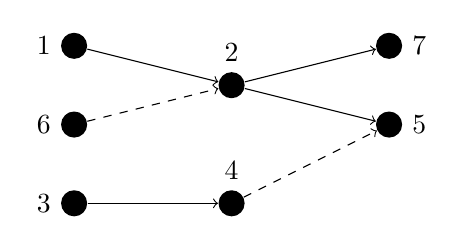
\begin{tikzpicture}[x=2cm]
                            \node[circle, fill=black, label=left:1] (1) at (0, 0) {};
                            \node[circle, fill=black, label=above:2] (2) at (1, -0.5) {};
                            \node[circle, fill=black, label=left:3] (3) at (0, -2) {};
                            \node[circle, fill=black, label=above:4] (4) at (1, -2) {};
                            \node[circle, fill=black, label=right:5] (5) at (2, -1) {};
                            \node[circle, fill=black, label=left:6] (6) at (0, -1) {};
                            \node[circle, fill=black, label=right:7] (7) at (2, 0) {};
                            \draw
                            (1) edge[->] (2)
                            (2) edge[->] (5)
                            (2) edge[->] (7)
                            (3) edge[->] (4)
                            (4) edge[->, dashed] (5)
                            (6) edge[->, dashed] (2);
                        \end{tikzpicture}
                    \end{minipage}
                \end{center}
            \subsubsection*{Algorithm Analysis}
                Given we have some problem $P$, and $S$ for all the possible solutions for $P$. In this course,we only consider the time complexity. A harder, more theoretical question, would be "can we improve our existing algorithm, or have we found the best algorithm for $P$?". In order to reason about this, we need to consider ehat is the least amount of work every member of $S$ must to do solve $P$ - this gives us a lower bound time complexity on $P$. This is important as we're not just considering a large amount of solutions, but all possible solutions that exist.
                \medskip

                For this, we will examine searching, and sorting algorithms; because these are frequently used (therefore efficiency is very important), and analysis for them have already been carried out (such that we know the optimal algorithms). If we can prove an algorithm has the complexity exactly on the lower bound, then we've proven that it's the best possible algorithm.
            \subsubsection*{Unordered List}
                Consider a list of elements (that allows for random access) $L$, and some target element $x$. We can consider a simple, linear approach; inspect each element, until the end of the list. For this, we have a best case of 1 (where it's the first item we check), and a worst case of $n$ (where the item is either at the end of the list, or not in the list at all). Note that here we are counting comparisons.
                \medskip

                In worst case analysis, we denote it with $W(n)$, which is the largest number of comparisons for an input size $n$. We could also consider the average case, which is $A(n)$, however this is much harder to analyse as we might need to know (or make an assumption) about its probability distribution.
                \medskip

                Here, let us reason about how linear search is optimal for an unordered list. Take any $A$ which solves the search problem. We can claim that if $A$ says the item isn't found, it must've inspected every element. In order to prove this by contradiction, suppose that $A$ didn't inspect $L[k]$, which is an arbitary index in the list. Now place some item, $x$ into $L[k]$, and $A$ would then return that the item wasn't found, which is incorrect. Therefore, in the worst case, $n$ comparisons are needed.
        \subsection*{14th February 2019}
            \subsubsection*{Ordered List}
                If the problem were now changed to be searching an ordered list, linear search would still be applicable, but no longer optimal.
                \medskip

                We can now consider binary search, which divides the list (and we're able to do that due to the ordered nature of the list). It can either be represented by pseudocode (which is trivial to work out), or as the following decision tree. Note that for sake of time, and because I'm lazy, if it goes down the right left hand side, for some node $n$, it means that $x < L[n]$, and for the right hand side, it would mean that $x > L[n]$. If $x = L[n]$, then we've solved it (note that the leaf nodes represent my result in this exam);
                \begin{center}
                    \begin{tikzpicture}
                        \node[] (o) at (0, 0) {3};
                        \node[] (ol) at (-2, -1.5) {1};
                        \node[] (or) at (2, -1.5) {5};
                        \node[] (oll) at (-3, -3) {0};
                        \node[] (olr) at (-1, -3) {2};
                        \node[] (orl) at (1, -3) {4};
                        \node[] (orr) at (3, -3) {6};
                        \node[] (olll) at (-3.5, -4.5) {fail};
                        \node[] (ollr) at (-2.5, -4.5) {fail};
                        \node[] (olrl) at (-1.5, -4.5) {fail};
                        \node[] (olrr) at (-0.5, -4.5) {fail};
                        \node[] (orll) at (0.5, -4.5) {fail};
                        \node[] (orlr) at (1.5, -4.5) {fail};
                        \node[] (orrl) at (2.5, -4.5) {fail};
                        \node[] (orrr) at (3.5, -4.5) {7};
                        \node[] (orrrl) at (3, -6) {fail};
                        \node[] (orrrr) at (4, -6) {fail};
                        \draw
                        (o) -- (ol)
                        (o) -- (or)
                        (ol) -- (oll)
                        (ol) -- (olr)
                        (or) -- (orl)
                        (or) -- (orr)
                        (oll) -- (olll)
                        (oll) -- (ollr)
                        (olr) -- (olrl)
                        (olr) -- (olrr)
                        (orl) -- (orll)
                        (orl) -- (orlr)
                        (orr) -- (orrl)
                        (orr) -- (orrr)
                        (orrr) -- (orrrl)
                        (orrr) -- (orrrr);
                    \end{tikzpicture}
                \end{center}
                We can say that the worst case, $W(8) = 4$, as it's the depth of the decision tree. However, this is a big improvement on linear search, as we are reducing the worst case to a logarithm of $n$, where the difference would be much more apparent in larger data sets. Since the worst case of binary search is the depth of the tree, we can say that it's the optimal solution.
                \medskip

                While we can fairly easily see the worst case by looking at the decision tree, it's not as apparent for other algorithms, or larger sets of data. We can use a recurrence relation to solve it;
                \begin{align*}
                    W(1) & = 1 \\
                    W(n) & = 1 + W(\floor{\frac{n}{2}})
                    \intertext{We can solve this by repeated expansion;}
                    W(n) & = 1 + W(\floor{\frac{n}{2}}) \\
                    & = 1 + [1 + W(\floor{\frac{n}{4}})] \\
                    & = 1 + 1 + 1 + W(\floor{\frac{n}{8}})] \\
                    & \phantom{=\ \ } ... \\
                    & = 1 + ... + 1 + W(1)
                \end{align*}
                Now, we can say that the number of 1s is the number of times the number is divisible by 2, hence $k$ where $2^k \leq n < 2^{k + 1}$. Therefore $k = \floor{\text{log}_2(n)}$, Hence it follows that $W(n) = 1 + \floor{\text{log}_2(n)}$.
                \medskip

                We can represent search algorithm, considering comparisons, as a binary tree - we either have the item being less than, greater than, or equal. In the latter, we can just terminate the algorithm. We can propose that if a binary tree has depth $d$, then it has $\leq 2^{d + 1} - 1$ nodes. This can be proven by induction over natural numbers.
                \medskip

                Given that the worst case performance of some search algorithm $A$ is $d + 1$ (where $d$ is the depth, and we can use the inequality for the nodes above). It follows that $d + 1 \geq \text{log}(n + 1)$ by taking logs of both sides. And this can be proven to be $W(n)$.
            \subsubsection*{Orders}
                Suppose we have some algorithm $W(n) = 7n^3 + 1000n + 32$, as $n$ gets larger, $7n^2$ is the most important term. If we ignore the constant $W(n)$ therefore has order $n^2$. We prefer algorithms of lower order, even if a higher order algorithm may have a lower operation time for small $n$. The constant factor can also be ignored.
                \medskip

                The main types of orders we encounter are; polynomial, exponential, and logarithmic. The heirachy for logarithmic (with polynomial) is as follows;
                \begin{center}
                    1 \ \ log($n$) \ \ $n$log($n$) \ \ $n^2$ \ \ $n^2$log($n$)
                \end{center}
                Let two functions $f, g : \mathbb{N} \mapsto \mathbb{R}^+$;
                \begin{itemize}
                    \itemsep0em
                    \item $f$ is $O(g) \leftrightarrow \exists m \in \mathbb{N} \exists c \in \mathbb{R}^+ [\forall n \geq m [f(n) \leq c \cdot g(n)]]$
                    \item $f$ is $\Theta(g) \leftrightarrow f $ is $O(g)$, and $g$ is $O(f)$
                        \subitem the $\Theta$ means order
                \end{itemize}
                We know that matrix multiplication is a $O(n^3)$ problem, but there exists a lower bound of $\Theta(n^2)$.
        \subsection*{18th February 2019}
\end{document}
